\chapter{Konvergence trajektorií}
Jak již bylo naznačeno v úvodní kapitole, v některých případech používáme ke
zlepšení energie aktuální trajektorie backtracking. Nicméně realizovat
backtracking trajektorii až úplně zpět k ústí tunelu by bylo výpočetně velmi náročné
a neefektivní, proto chceme nějakým způsobem backtracking napojit na již
spočítanou trajektorii, čímž si často můžeme ušetřit značné množství práce a hlavně
takto dokážeme snížit energii trajektorie například v případě, že máme více úzkých
hrdel těsně po sobě. To ilustruje obrázek č. \ref{fig:two_bottlenecks}, na kterém
můžeme vidět, že se algoritmus nejprve dostane na řez č. 2 z pozice řezu č. 1
a musí spustit backtracking z konformace ligandu, která je vyobrazena na řezu č. 2.
S touto konformací pak pokračuje dále, avšak pokud během průchodu prostorem
mezi řezy 2 a 3 nedojde k rotaci, bude na řezu č. 3 opět potřeba spouštět
backtracking s opačnou rotací, avšak ten ve chvíli, kdy dospěje na řez č.2,
pravděpodobně selže.

\begin{figure}[ht]
\centering
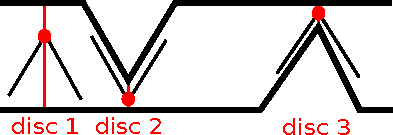
\includegraphics[width=.5\hsize]{img/two_bottlenecks.pdf}
\caption{Schématický 2D pohled na situaci se dvěma úzkými hrdly.}
\label{fig:two_bottlenecks}
\end{figure}

Uvažme tedy, že máme pozici backtracking trajektorie $ \tilde{\lambda}^i $
na řezu $ \theta_i $ a pozici dopředné trajektorie $ \lambda^i $ na tomtéž řezu.
Nejjednodušším přístupem v takové situaci je zkontrolovat, zda platí
$ \tilde{\lambda}^i \in \Delta \lambda^i $. Tuto kontrolu můžeme provádět v každé
iteraci backtrackingu, neboť při ní stačí lineárně projít všechny atomy ligandu
a zkontrolovat jejich vzdálenosti oproti ligandu dopředné trajektorie. Ligandy
navíc typicky mívají velmi malý počet atomů, takže se skutečně jedná o nenáročný
výpočet. Tento přístup bude fungovat ve chvíli, kdy molekula ligandu po opuštění
úzkého hrdla zkonverguje do původní konformace, kterou zaujímá ligand v dopředné
trajektorii, k čemuž dojde zejména v situaci, kdy existuje lokální energetické
minimum, do kterého se z backtracking konformace můžeme dostat gradientním sestupem.
Této situaci budeme říkat \textit{jednoduchá konvergence}.

\begin{figure}[ht]
\centering
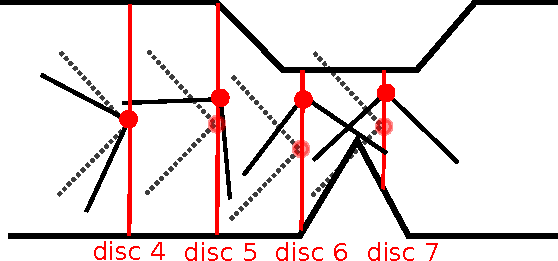
\includegraphics[width=.5\hsize]{img/backtracking_simple.pdf}
\caption{Jednoduchá konvergence. Dopředná trajektorie je vyznačena tečkovaně,
backtracking plnou čárou.
}
\label{fig:simple_convergence}
\end{figure}


Příklad takové situace můžeme vidět na obrázku č. \ref{fig:simple_convergence}.
Při dopředném pohybu jsme uvázli v úzkém hrdle, ze kterého jsme s vhodnější
konformací spustili backtracking, který po několika iteracích na disku č. 4
samovolně zkonvergoval do pozice téměř identické s pozicí dopředné trajektorie.
V tuto chvíli by byl backtracking ukončen a dále bychom pokračovali z disku č. 7.
Poznamenejme, že uvedený obrázek je čistě schématický a konvergenční proces
by v praxi zabral více kroků kvůli požadavkům na spojitost.

Jednoduchá konvergence může dobu výpočtu zkrátit, nicméně v praxi se často stává,
že ligand při backtrackingu zkonverguje do konformace, která je velmi podobná
konformaci dopředné trajektorie, ale liší se například rotací. Obě pozice tak
mohou mít velice podobnou energii, ale z mělkého lokálního minima se bez pomoci
nedostanou a backtracking by mohl dospět až k ústí tunelu.

\begin{figure}[ht]
\centering
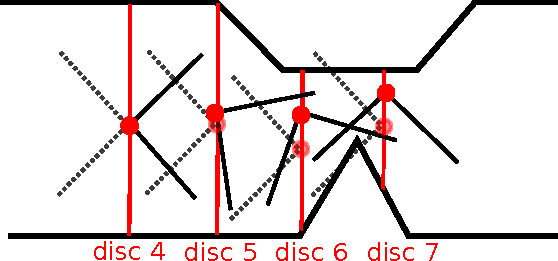
\includegraphics[width=.5\hsize]{img/backtracking_bad_rotation.pdf}
\caption{Obrázek zachycuje situaci, ve které při backtrackingu dojde k opačné
rotaci ligandu, která v důsledku znemožní aplikaci jednoduché konvergence.
Dopředná trajektorie je vyznačena tečkovaně, backtracking plnou čárou.
}
\label{fig:backtracking_bad}
\end{figure}

Schéma č. \ref{fig:backtracking_bad} je ukázkou takové konstelace, ve které
oproti předchozímu příkladu při backtrackingu došlo k opačné rotaci ligandu
a algoritmus se tím dostal do jiného lokálního energetického minima. Obě situace
mohou nastat, neboť dokovací algoritmus je náhodnostní a můžeme z něj ve stejné
situaci na disku č. 6 dostat různý iniciální krok backtrackingu.

Aby náš algoritmus v situaci, ke které dojde na řezu č. 4, mohl využít již spočítanou
dopřednou trajektorii, musíme zjistit, zda mezi pozicemi ligandu z backtracking trajektorie
$ \tilde{\lambda}^4 $ a dopředné trajektorie $ \lambda^4 $ neexistuje nějaká silná
energetická bariéra, která by v reálném systému činila pravděpodobnost přechodu
mezi těmito pozicemi nulovou. To podobně jako u v úvodu zmíněné optimalizace
energie ligandu budeme realizovat vypočtením dílčí spojité trajektorie.
V tomto případě ale půjde o spojitou trajektorii mezi pozicí $ \lambda^i $ dopředné
trajektorie a pozicí $ \tilde{\lambda}^i $ z backtracking algoritmu. Takový
výpočet je o něco obtížnější, neboť vedle aplikace omezujícího vzoru (kvůli
požadavku na spojitost) musíme ještě nějakým způsobem zajistit, abychom v průběhu
výpočtu atomy výchozího ligandu $ a_c \in \lambda^i $ tlačili
směrem ke korespondujícím atomům cílového ligandu $ \tilde{a}_c \in \tilde{\lambda}^i $.
Tento proces budeme nazývat aplikace \textit{slabého omezujícího vzoru} (nebo
zkráceně \textit{slabého vzoru}) a jeho implementaci si nastíníme v následující
sekci \ref{subsec:weak_pattern}, na kterou navážeme podkapitolou
\ref{subsec:convergence_algorithm} věnovanou samotnému konvergenčnímu algoritmu.




\section{Slabý omezující vzor} \label{subsec:weak_pattern}
Implementace omezujících vzorů tak, aby fungovaly v souladu s našimi požadavky,
je poměrně komplikovaná, a proto zde popíšeme jen ty části, které jsou nezbytné
pro pochopení konvergenčního algoritmu. Omezující vzory v principu fungují tak,
že atomům ligandu, které jsou mimo pozici požadovanou vzorem, přiřazují
penalizační silový vektor, jehož velikost roste se vzdáleností od ideální pozice
a je orientován ve směru od současné $ \tilde{a}_c $ k ideální pozici daného
atomu $ \tilde{a}_c $. Přesněji řečeno penalizační vektor $ \vec{p_c} $ pro
atom $ c $ definujeme jako
\begin{align*}
    \vec{p_c} = \vec{v} \cdot \max\left\{ 0, 1 - \frac{\delta}{\norm{\vec{v}}} \right\},
\end{align*}
kde $ \vec{v} $ je směrový vektor daný korespondujícími atomy, tedy
$ \vec{v} = a_c - \tilde{a}_c $, a $ \delta $ je parametr spojitosti z úvodní
kapitoly. Jak vidno, vektor je buďto nulový, pokud je aktuální pozice atomu vzdálena
o méně nebo rovno $ \delta $, nebo do něj v opačném případě přiřadíme vektor
realizující rozdíl mezi atomy ponížený o $ \delta $.

Vektory $ p_c $ můžeme chápat jakožto evaluaci silového pole daného omezujícím
vzorem. Suma $ E = \sum \norm{p_c} $ reprezentuje potenciální energii
ligandu v dané pozici vzhledem k silovému poli omezujícího vzoru. Energii $ E $
a vektory $ p_c $ pak použijeme v dokovacím algoritmu jako informace o jednom
ze silových polí působících na ligand. Tento algoritmus se snaží minimalizovat sumu
potenciálních energií přes všechna silová pole a vektory $ p_c $ využívá pro
směřování výpočtu. Na tomto místě musíme poznamenat, že v praxi při výpočtu
je sice výpočet energie přesně takový, jak jsme jej popsali, nicméně při práci
se silovým vektorem omezujeme fixním způsobem jeho velikost, abychom do systému
velkými čísly nezanášeli numerickou nepřesnost. Při praktickém počítání se totiž
ukazuje, že velikost silového vektoru od určité hranice není relevantní a
je lepší ji omezit ve prospěch numerické přesnosti.


V případě silného omezujícího vzoru, který zajišťuje spojitost, bereme za
ideální pozici atomů výchozí pozici $ \lambda^i $, čímž budeme silně penalizovat atomy, které se
z původní pozice vzdálí o více než $ \delta $. Slabý omezující vzor bude naopak
atomy z výchozí pozice přitahovat k atomům backtracking trajektorie. Tato konfigurace
potřebuje ještě jednu drobnou úpravu, aby její funkcionalita odpovídala našemu
původnímu záměru, což byla implementace spojitého přesunu od dopředné trajektorie
k backtracking trajektorii. Chceme totiž primárně respektovat silný omezující
vzor, aby ligandy atomu nemohly přeskočit nějakou energetickou bariéru, a posun
ligandu je až sekundární optimalizační cíl. Tento požadavek zajistíme tím, že
potenciální energii i sílu ligandu v silovém poli slabého vzoru budeme v dokovacím
algoritmu započítávat s nižší váhou.





\section{Konvergenční algoritmus} \label{subsec:convergence_algorithm}
S použitím slabého vzoru je samotný algoritmus pro výpočet konvergenční
trajektorie poměrně přímočará záležitost a zachycuje jej pseudokód č.
\ref{alg:convergence}. Algoritmus v každé iteraci nejprve na řádku
\ref{alg:convergence:docking} zavolá dokovací proceduru se silným omezujícím
vzorem $ \alpha(\lambda) $ a slabým vzorem $ \beta(\tilde{\lambda})$. Dokovací
procedura vrátí jednu nebo více nových konformací, ze kterých vybereme
tu nejlepší přípustnou variantu, pokud nějaká existuje.

Aby byla pozice přípustná,
musí v první řadě splňovat podmínku spojitosti $ \lambda' \in \Delta\lambda $.
Spojitost je potřeba kontrolovat proto, že pomocí omezujících vzorů dokovací algoritmus
pouze nějakým způsobem směrujeme, avšak v praxi se může stát, že se atomy ligandu
pokoušíme natlačit příliš blízko k atomům proteinu, čímž můžeme vynutit příliš
velký skok. S tím souvisí také druhá podmínka přípustnosti, která ověřuje, zda
se nesnažíme překonat příliš velkou energetickou bariéru. K tomu může docházet
například ve chvíli, kdy se pokoušíme implementovat konvergenční trajektorii
v příliš úzkem místě (příklad takové situace můžeme vidět na obrázku č.
\ref{fig:narrow_tunnel}). Prakticky pak porovnáváme celkovou potenciální energii
ligandu $ E(\lambda') $ se zadaným parametrem maximální energie $ E_{max} $.
Tento parametr může být nastaven například na energii ligandu, která nás vedla ke
spuštění backtrackingu (ujistíme se tak, že backtracking s konvergencí nepovedou
k většímu energetickému maximu, než potenciální dopředná trajektorie). Kontrolu
přípustnosti implementujeme na řádku č. \ref{alg:convergence:feasibility}.

\begin{figure}[ht]
\centering
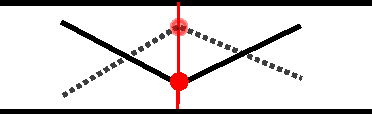
\includegraphics[width=.5\hsize]{img/narrow_tunnel.pdf}
\caption{Schématický 2D obrázek ve kterém konvergenční algoritmus narazí na
silnou energetickou bariéru, za předpokladu, že ligand není flexibilní (úhel
svíraný jeho atomy mezi sebou se nemůže změnit)}
\label{fig:narrow_tunnel}
\end{figure}

Vývoj algoritmu měříme v metrice průměrné vzdálenosti od cílové pozice
ligandu. Přesněji používáme funkci
$ \operatorname{AvgDst}(\lambda, \tilde{\lambda})
    = \frac{\mathlarger{\sum}\norm{a_j - b_j}}{|\lambda|} $, kde $ a_j \in \lambda $,
$ b_j \in \tilde{\lambda} $ jsou pozice atomů a $ |\lambda| $ značí počet atomů ligandu.
V této metrice jednak vybíráme nejlepší pozici ligandu z pozic aktuální iterace
(konkrétně se jedná o podmínku na řádku \ref{alg:convergence:best}) a druhak
pomocí ní na řádku \ref{alg:convergence:progress} kontrolujeme, zda se algoritmus
posouvá směrem k cílové pozici. Pokud se nám během jedné iterace nepodaří průměrnou
vzdálenost zlepšit, algoritmus končí a vyhlásí, že konvergence selhala a je ji
potřeba spustit z jiné pozice backtracking trajektorie.

Výpočet úspěšně ukončíme pokud platí $\lambda \in \Delta\tilde{\lambda}$ a
vrátíme vypočítanou konvergenční trajektorii $ \tau $.

\begin{algorithm}
\caption{Výpočet konvergenční trajektorie}
\label{alg:convergence}
\begin{algorithmic}[1]

\Function{convergence}{$ \lambda, \tilde{\lambda} $}
    \State $ \tau = [\,] $
    \While {$\lambda \not\in \Delta\tilde{\lambda}$}
        \State $ L \gets $ Conformations found by docking algorithm using $ \alpha(\lambda) $
            and $ \beta(\tilde{\lambda})$ \label{alg:convergence:docking}
        \State $ d \gets \operatorname{AvgDst}(\lambda, \tilde{\lambda}) $
        \For{$ \lambda' \in L $}
            \If {$ \lambda' \in \Delta\lambda \wedge E(\lambda') \leq E_{max}$} \label{alg:convergence:feasibility}
                \If {$ \operatorname{AvgDst}(\lambda', \tilde{\lambda})
                        < \operatorname{AvgDst}(\lambda, \tilde{\lambda}) $} \label{alg:convergence:best}
                    \State $ \lambda \gets \lambda' $
                \EndIf
            \EndIf
        \EndFor
        \If {$ \operatorname{AvgDst}(\lambda, \tilde{\lambda}) < d $} \label{alg:convergence:progress}
            \State $d \gets \operatorname{AvgDst}(\lambda, \tilde{\lambda}) $
            \State $ \operatorname{append}(\tau, \lambda) $
        \Else
            \State \Return \textbf{Failed}
        \EndIf
    \EndWhile
    \State \Return $\tau$
\EndFunction


\end{algorithmic}
\end{algorithm}
